\Exhibit{BeamGitHubStars}{%
    Скриншот топ 1.2\% репозиториев \Asf, среди которых Beam%
}

Это скриншот страницы GitHub со всеми репозиториями, принадлежащими \Asf.
Они отсортированы по количеству звёзд, начиная с самого большого.

Репозиторий `beam' виден внизу первой страницы, а всего страниц -- 85.
На этом скриншоте этот репозиторий 30-й по количеству звёзд.

Звёзды GitHub -- это метрика популярности проекта, как поясняется в \ExhibitRef{GitHubStars}.

В адрес этого скриншота уже заложена сортировка по звёздам,
но это можно дополнительно проверить, выбрав `Sort' \textbackslash `Stars'
в выпадающем списке наверху страницы.

Примечание: К тому времени, когда вы будете проверять эту страницу, `beam' может съехать на вторую страницу.
Если его нет внизу первой страницы, пожалуйста, проверьте вторую тоже.

\begin{center}
    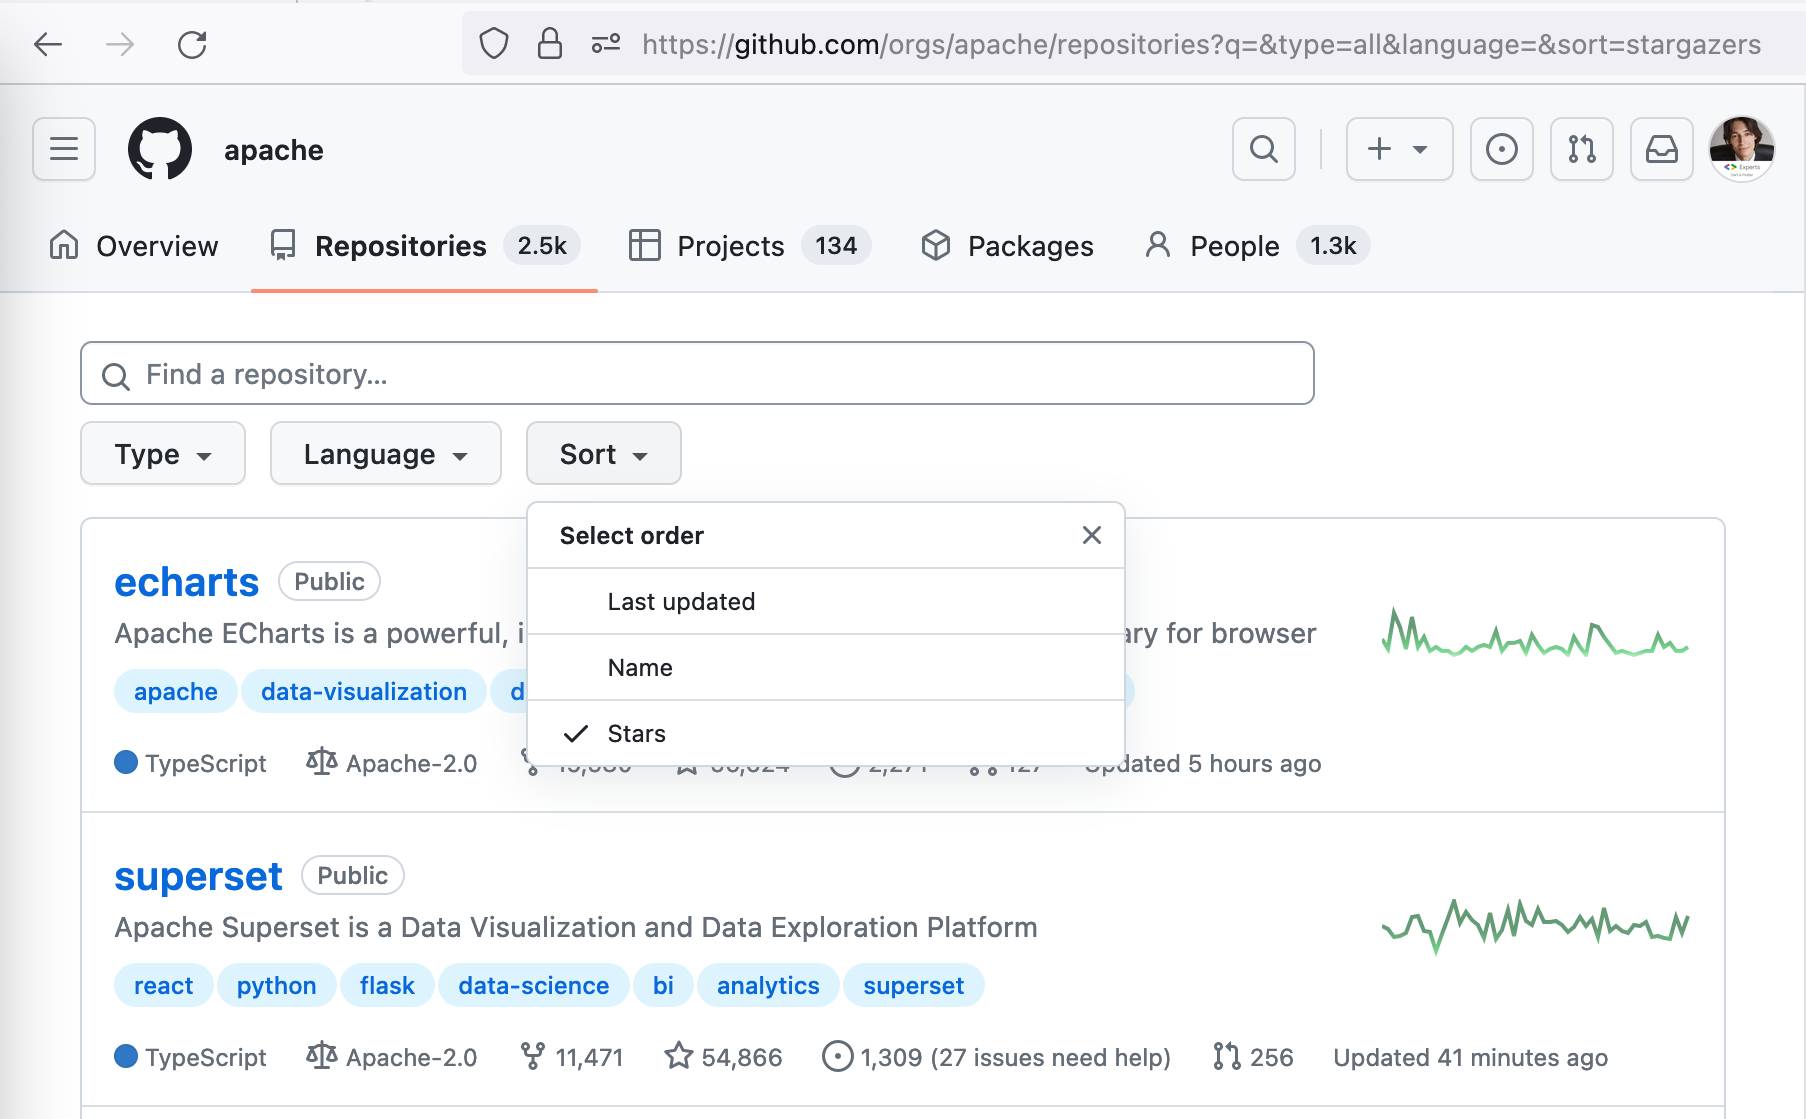
\includegraphics[width=40em]{beam-github-stars-dropdown-p1}
\end{center}
\WillContinue
\pagebreak

\Continuing
\begin{center}
    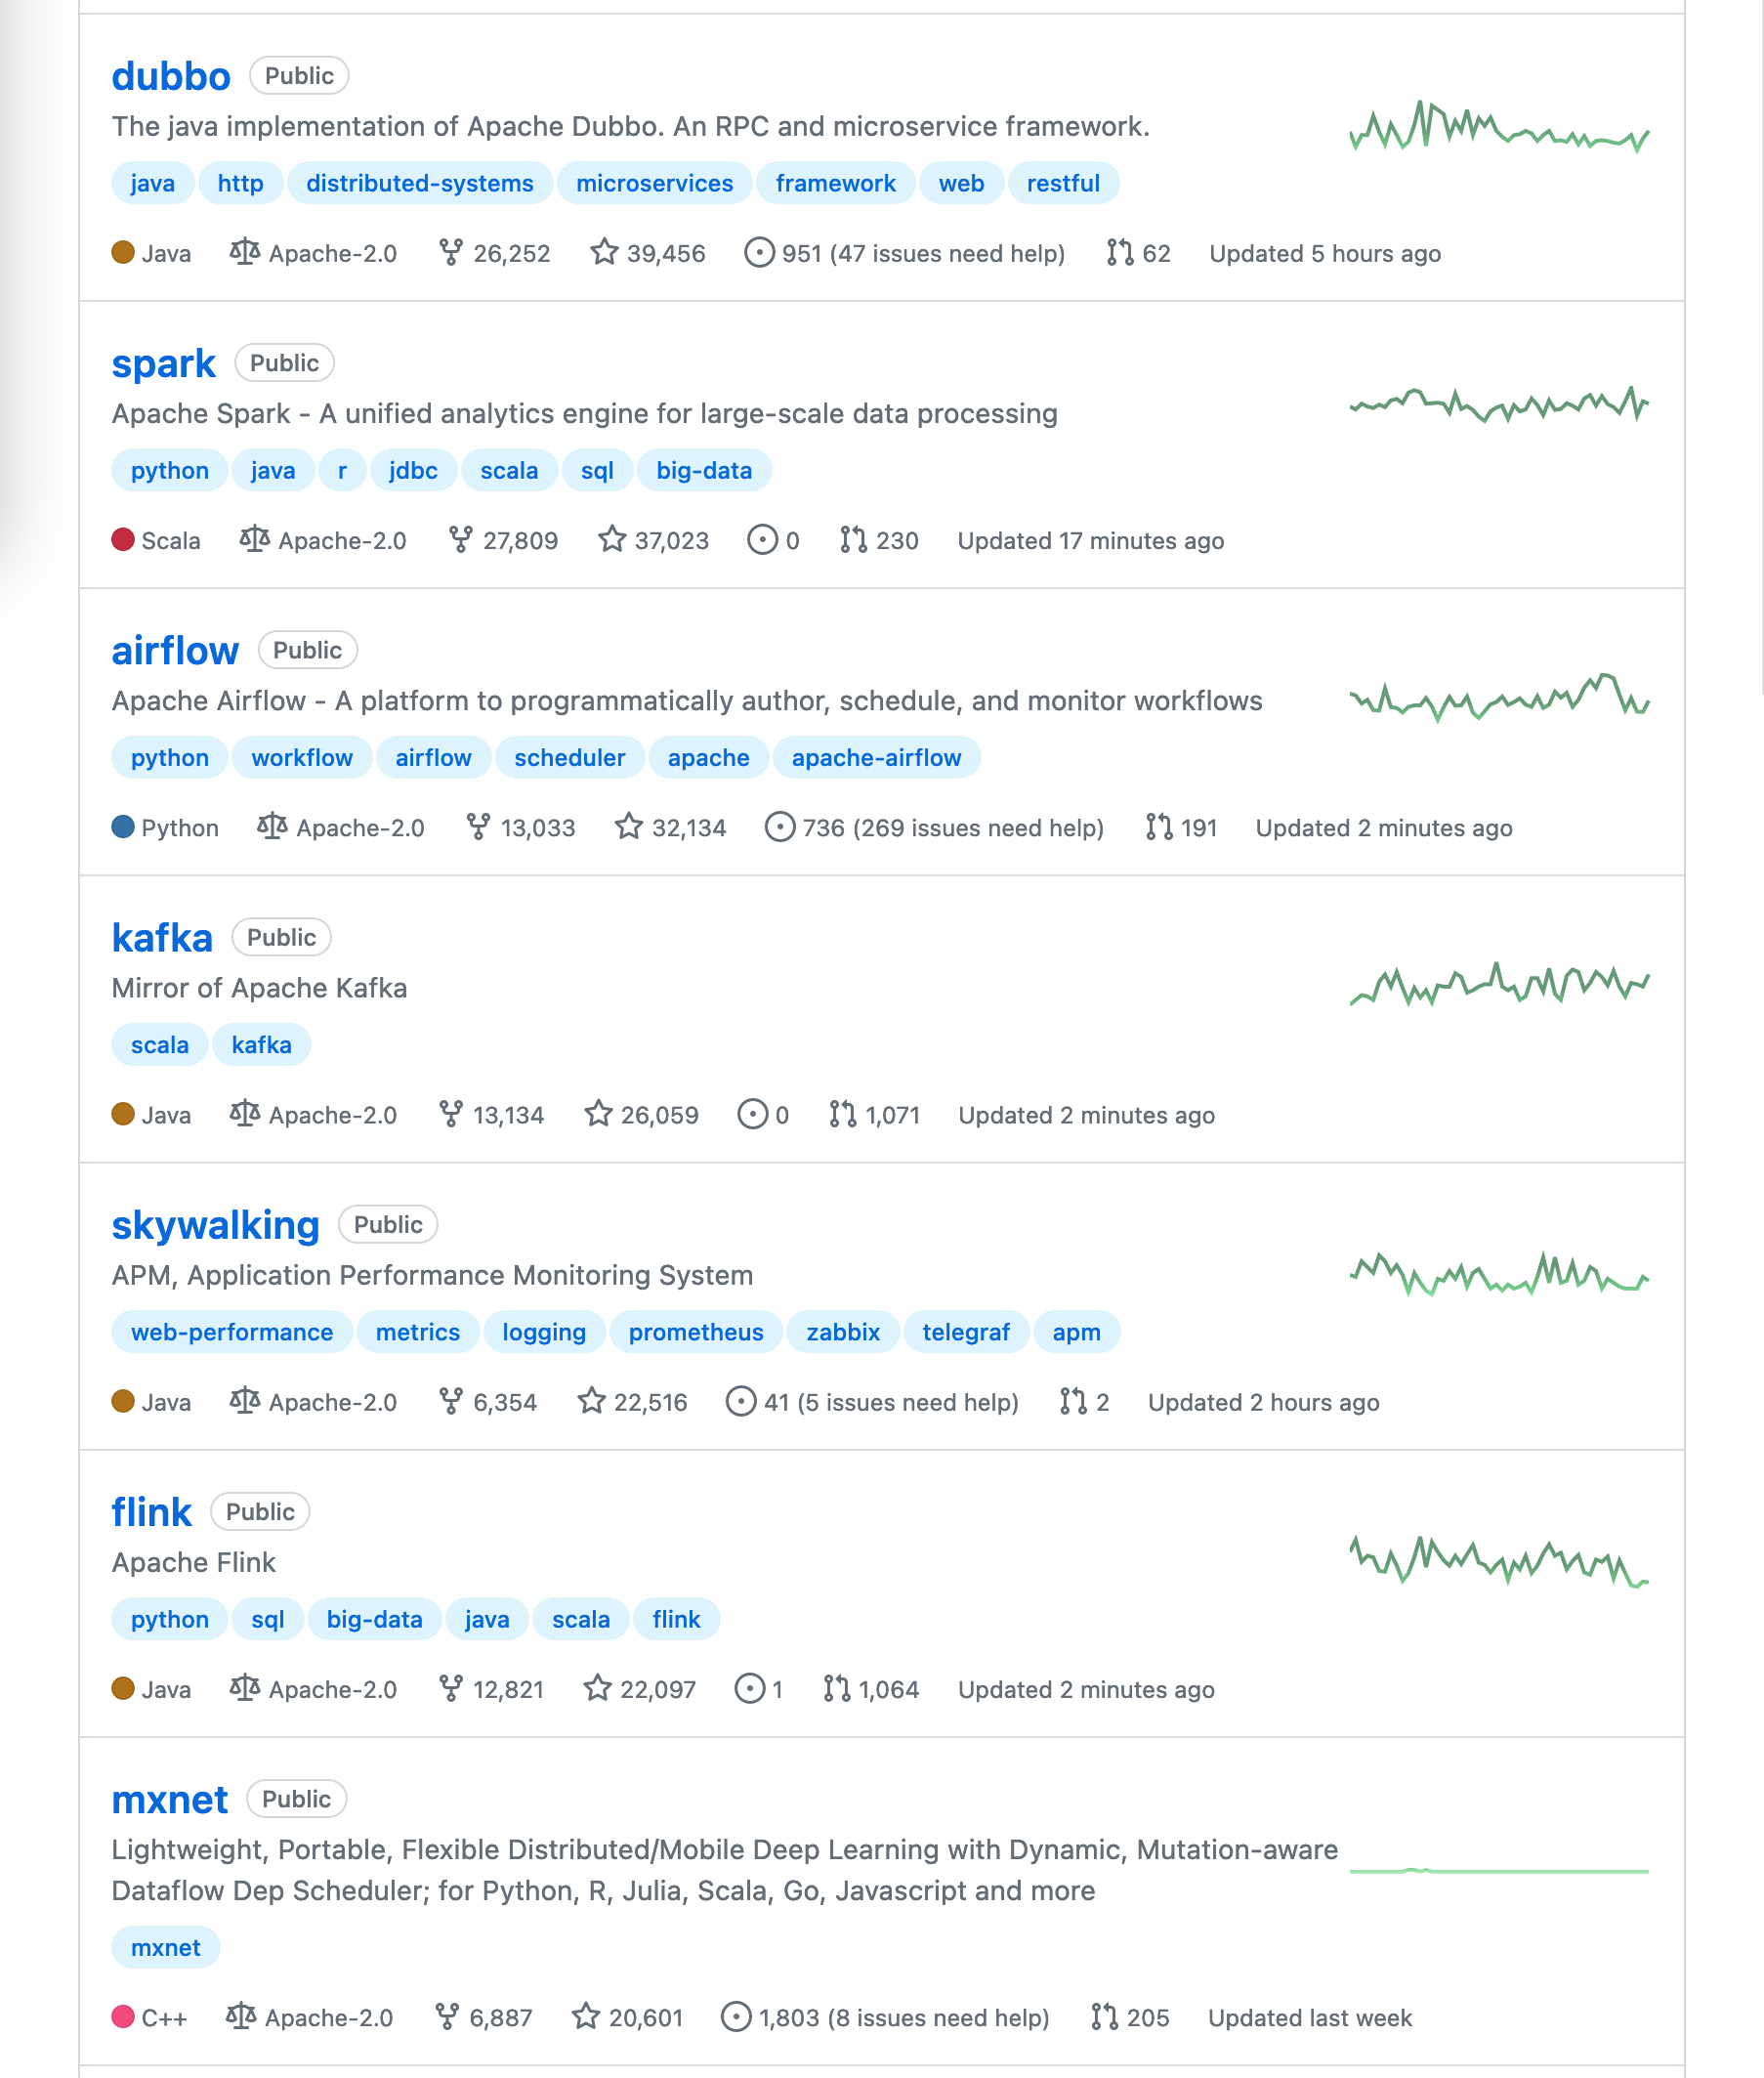
\includegraphics[width=40em]{beam-github-stars-dropdown-p2}
\end{center}
\WillContinue
\pagebreak

\Continuing
\begin{center}
    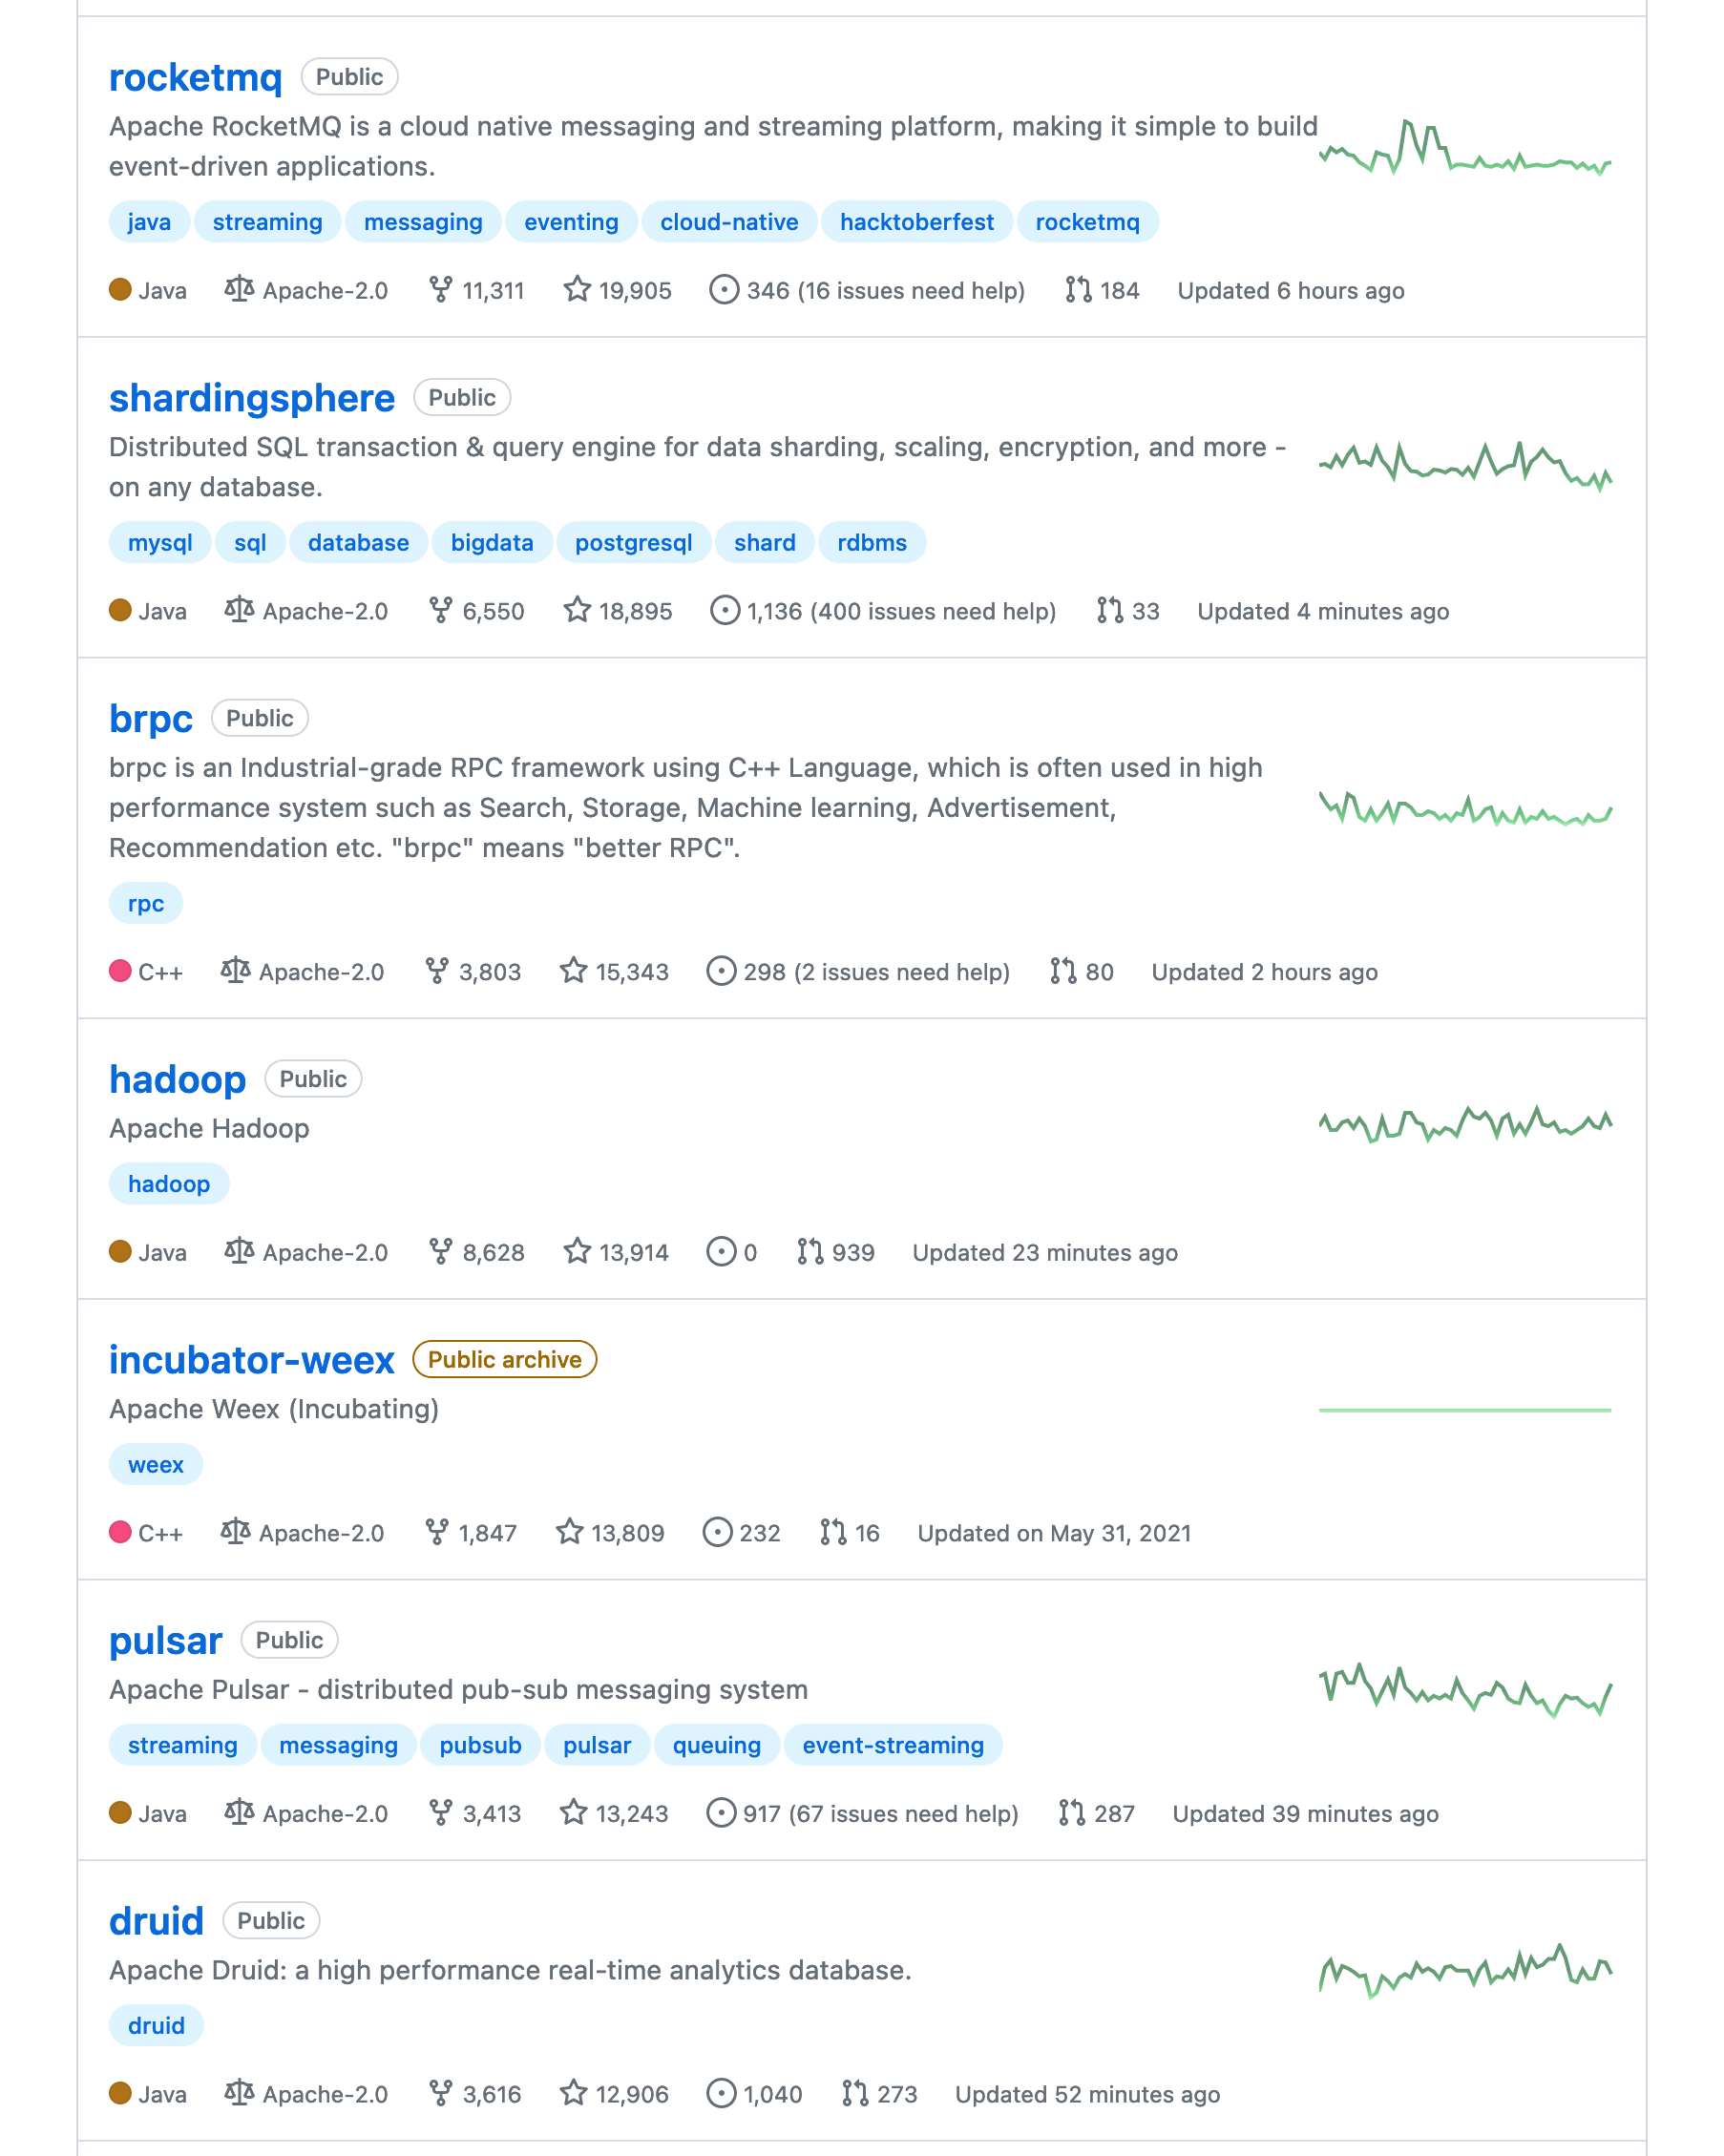
\includegraphics[width=40em]{beam-github-stars-dropdown-p3}
\end{center}
\WillContinue
\pagebreak

\Continuing
\begin{center}
    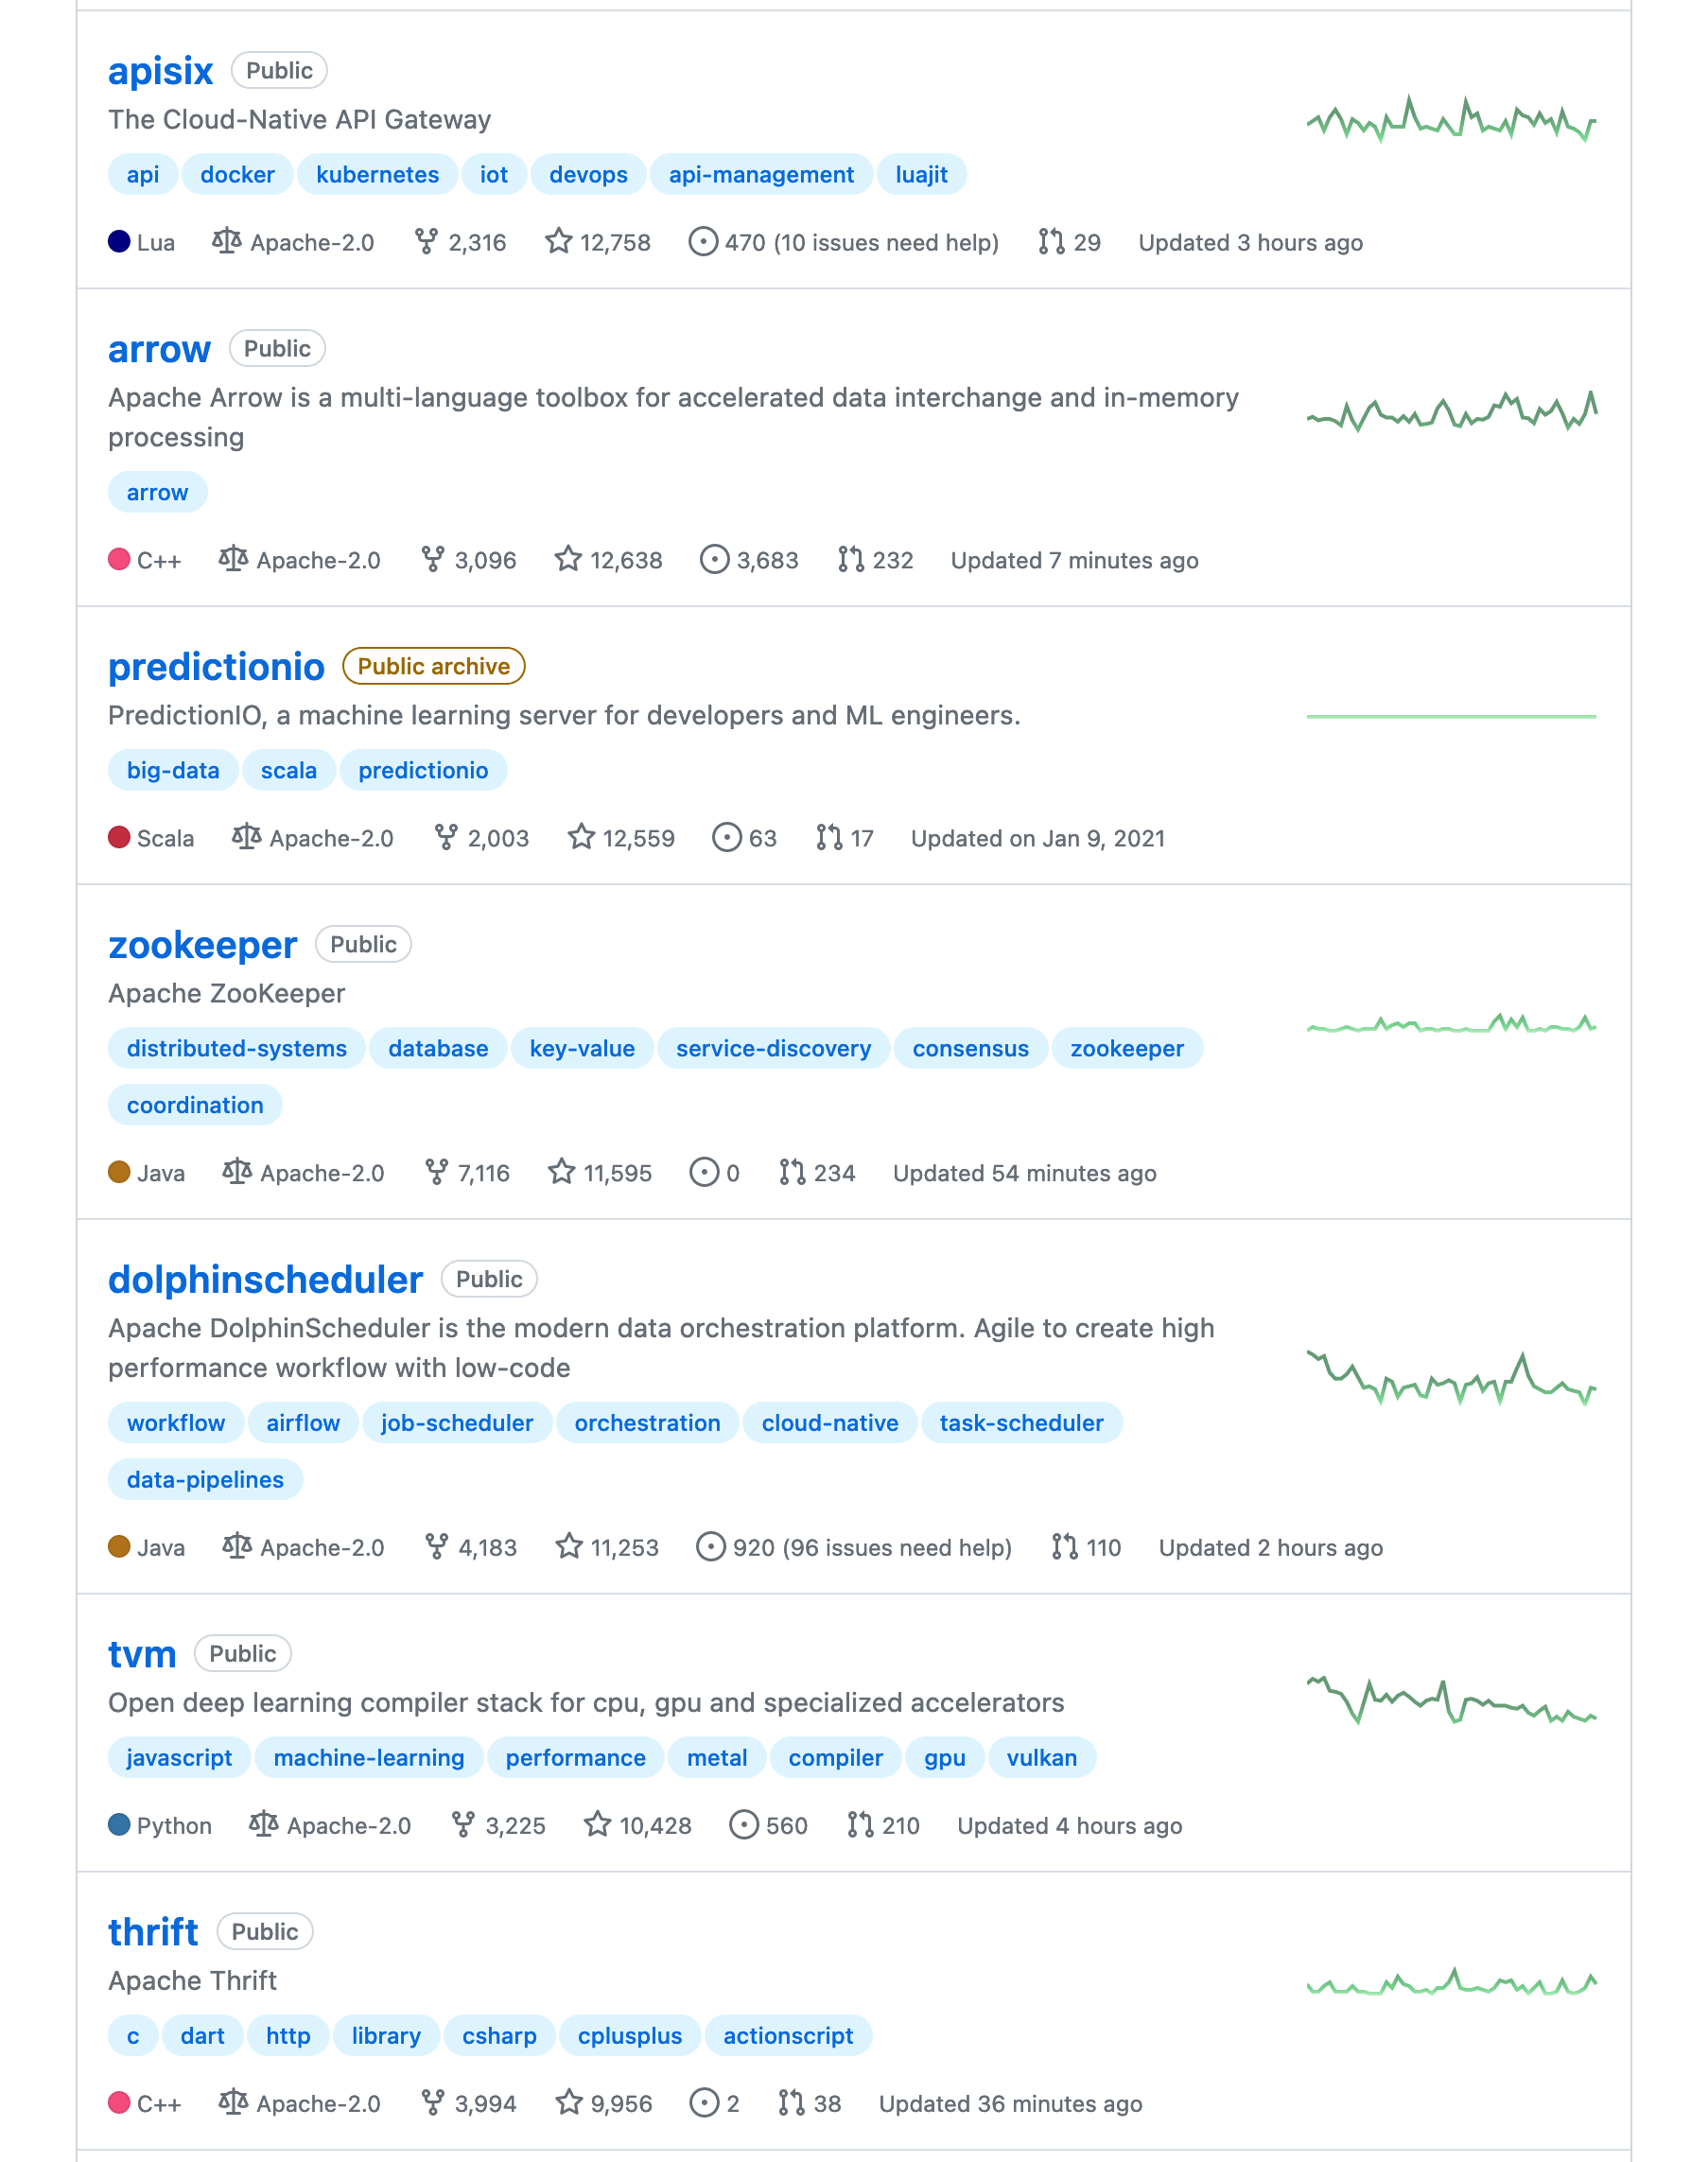
\includegraphics[width=40em]{beam-github-stars-dropdown-p4}
\end{center}
\WillContinue
\pagebreak

\Continuing
\begin{center}
    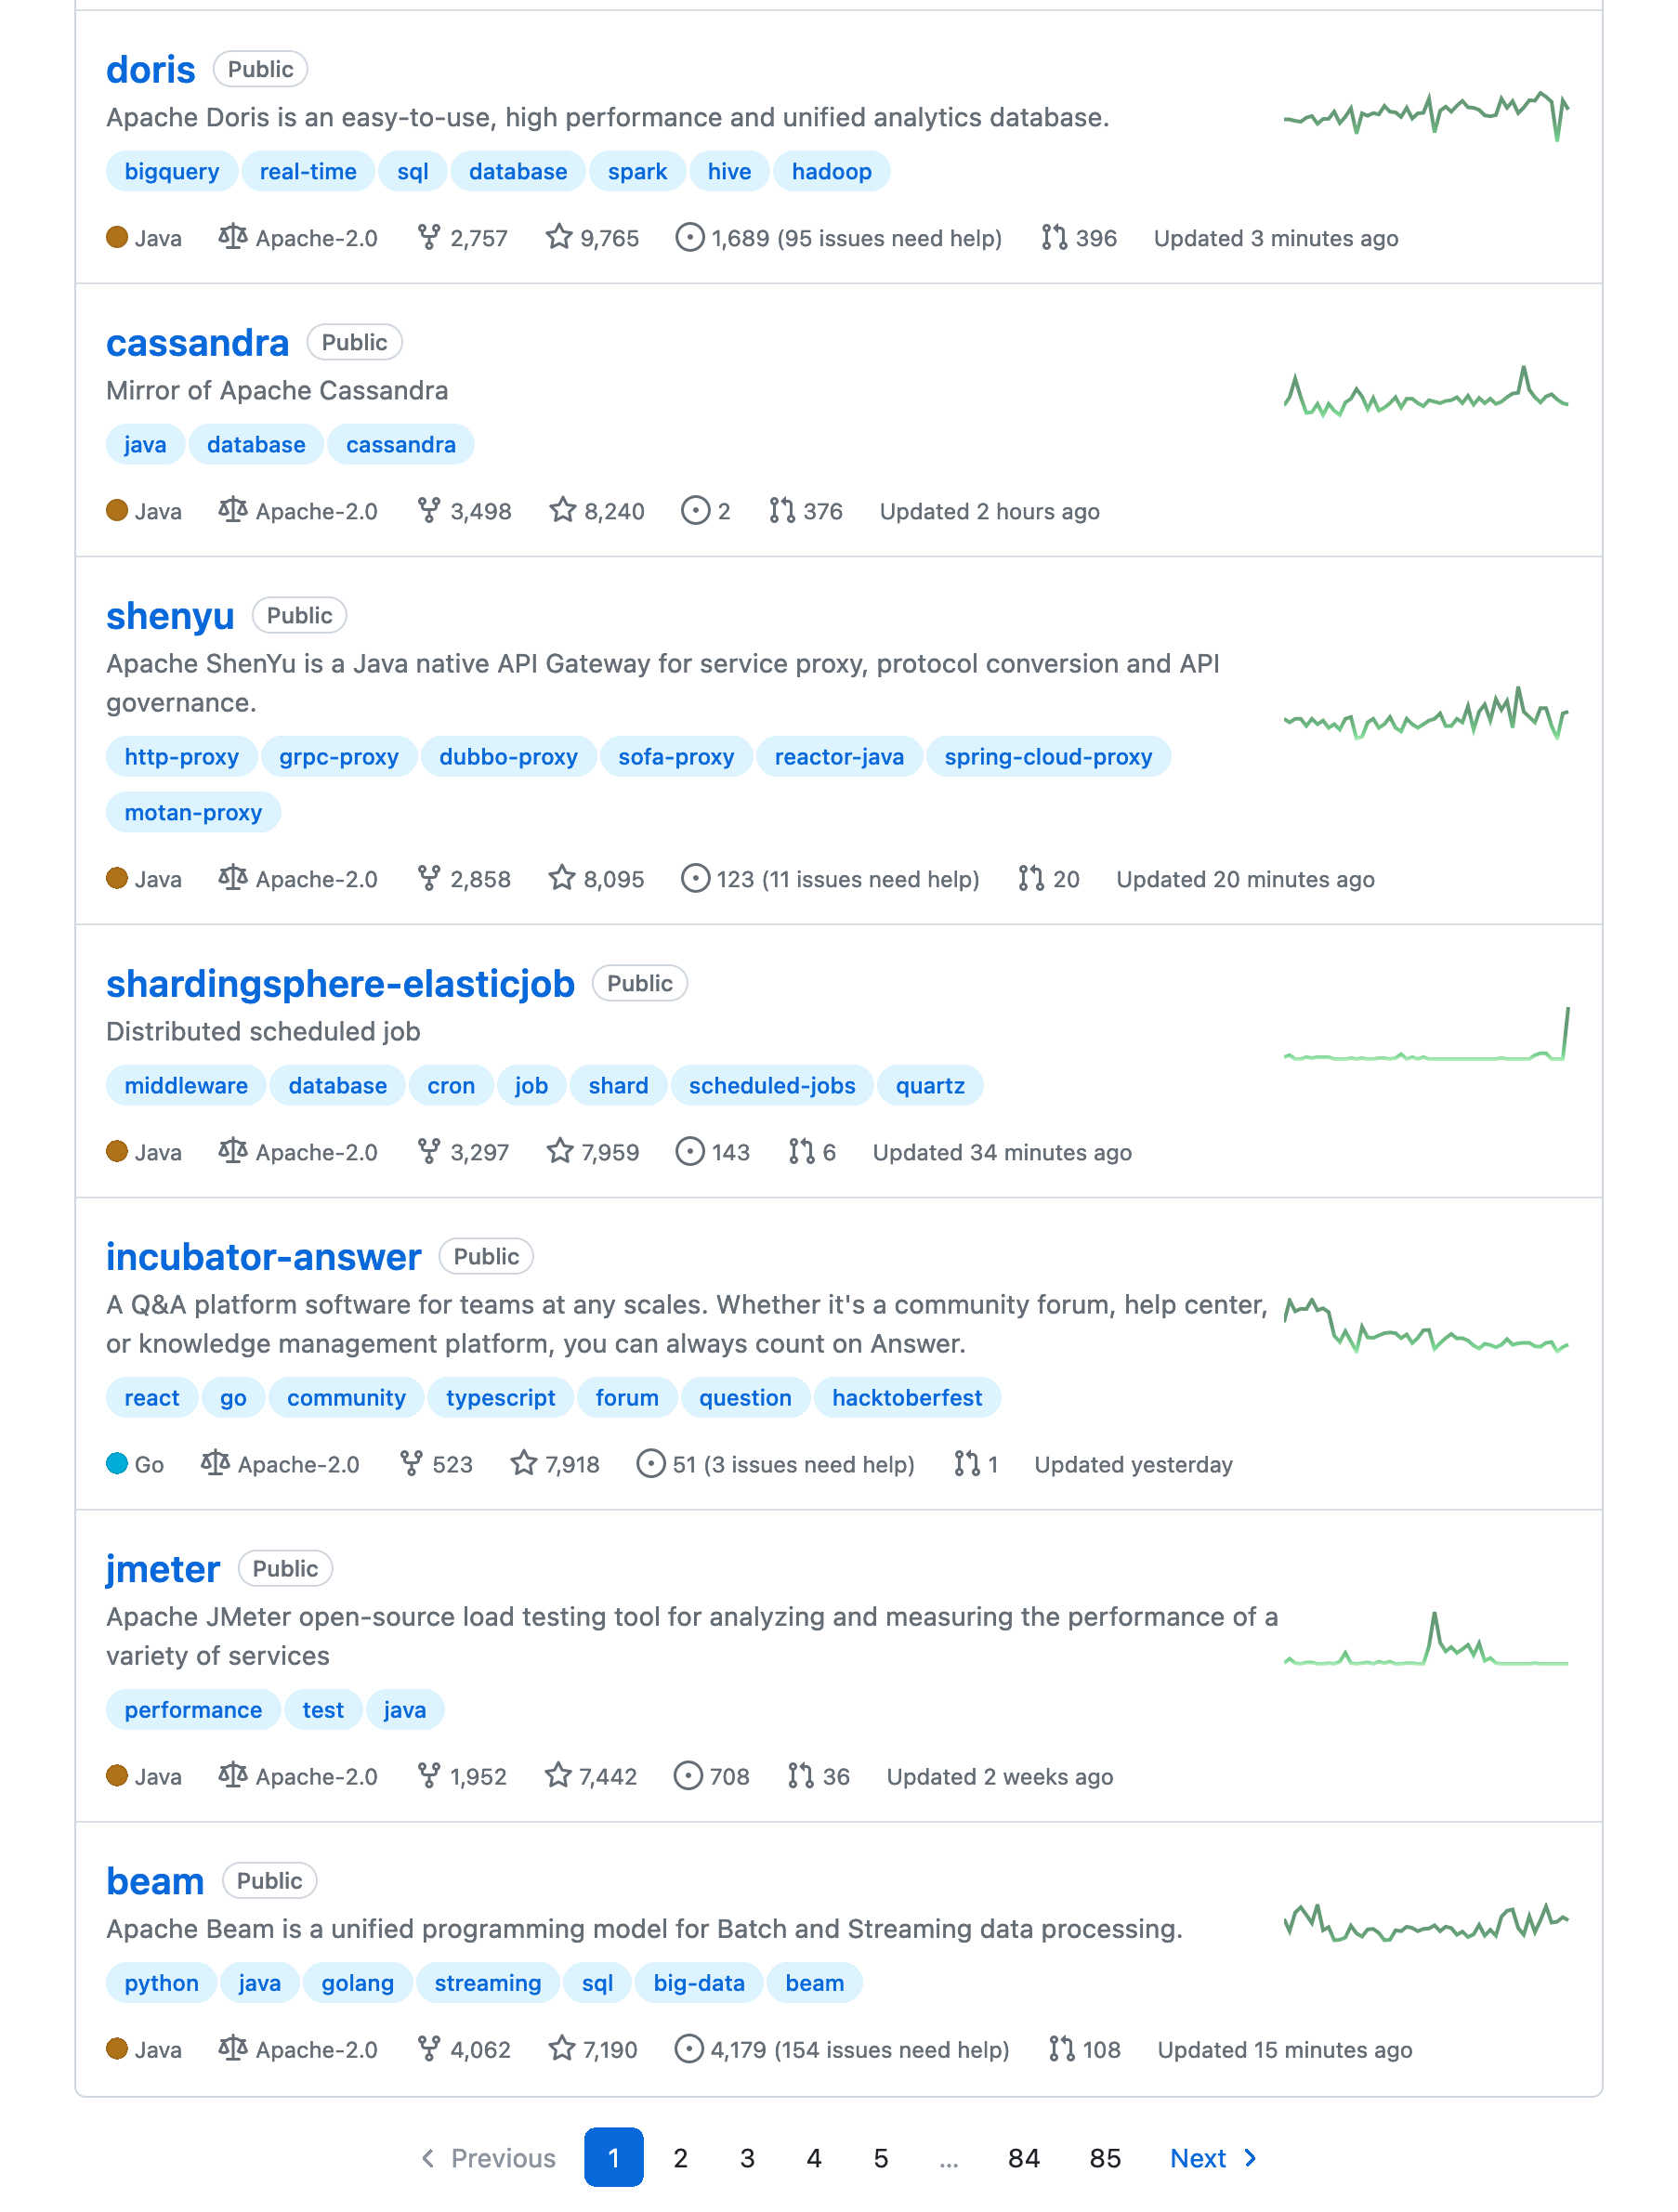
\includegraphics[width=40em]{beam-github-stars-dropdown-p5}
\end{center}

\pagebreak
